%%%%%%%%%%%%%%%%%%%%%%%%%%%%%%%%%%%%%%%%%%%%%%%%%%%
%% P3: Phenomenology of Particle Physics                         
%%
%% Author:  André Rubbia                   		 
%%
%% Figure 14.4 Schematic of the $g-2$ muon storage ring experiment.
%%
%% This work is licensed under the Creative Commons Attribution 4.0 International License. 
%% To view a copy of this license, visit http://creativecommons.org/licenses/by/4.0/ or 
%% send a letter to Creative Commons, PO Box 1866, Mountain View, CA 94042, USA.
%%
%%%%%%%%%%%%%%%%%%%%%%%%%%%%%%%%%%%%%%%%%%%%%%%%%%%

\documentclass[a4paper,10pt]{article}

\usepackage[T1]{fontenc}
\usepackage[utf8]{inputenc}
\usepackage{lmodern}
\usepackage[labelfont=bf]{caption}
\usepackage{upgreek}

\usepackage{tikz}
\usepackage{pgfplots}
\pgfplotsset{compat=1.17}
\usepgfplotslibrary{ternary}
\usepgfplotslibrary{fillbetween}
\usepgfplotslibrary{external}

\usepackage{braket}

\def\d{\mathrm{d}}

\pgfkeys{/pgf/number format/.cd,1000 sep={}}

\begin{document}

%%%%%%%%%%%%%%%%% FIGURE %%%%%%%%%%%%%%%%%%%%%%%%%%%%%%%%%%
\begin{figure}[htb]
\begin{center}
    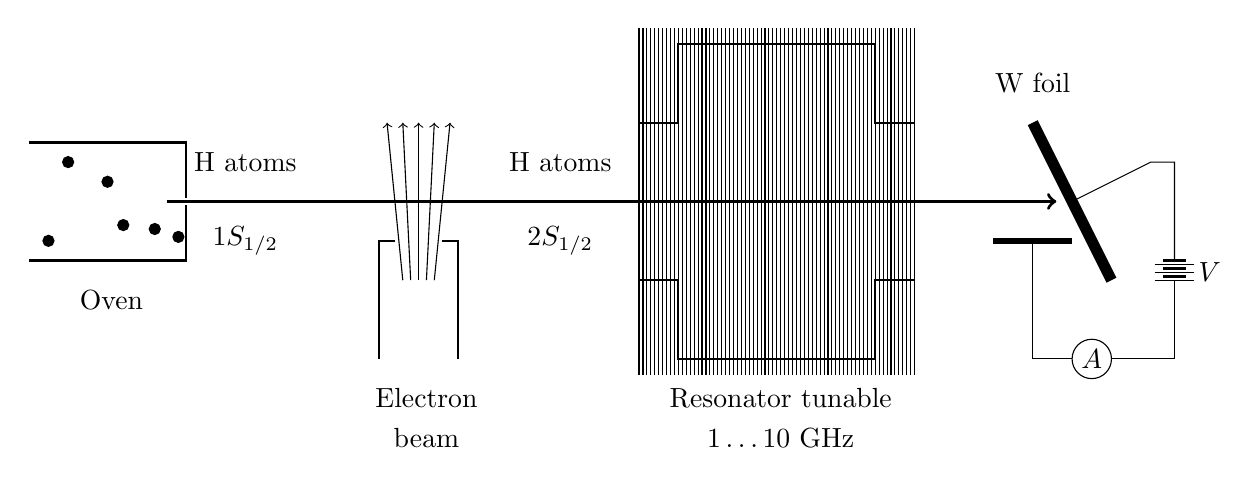
\begin{tikzpicture}[scale=1]
         \draw[thick] (-1.75,0.75) -- +(2,0.0) -- +(2,-0.7);
         \draw[thick] (-1.75,-0.75) -- +(2,0.0) -- +(2,+0.7);
         \draw[fill] (-1.5,-0.5) circle (2pt);
         \draw[fill] (-1.25,0.5) circle (2pt);
         \draw[fill] (-0.75,0.25) circle (2pt);
         \draw[fill] (0.15,-0.45) circle (2pt);
         \draw[fill] (-0.15,-0.35) circle (2pt);
         \draw[fill] (-0.55,-0.3) circle (2pt);
	\node at (-0.7,-1.25) {Oven};

	\node at (1, 0.5) {H atoms};
	\node at (1, -0.5) {$1 S_{1/2}$};
         \draw[very thick,->] (0.,0) -- +(11.3,0);

  \begin{scope}[shift={(3,0)}]
  \draw[->] (0,-1) -- +(-0.2,2);
  \draw[->] (0.1,-1) -- +(-0.1,2);
  \draw[->] (0.2,-1) -- +(0,2);
  \draw[->] (0.3,-1) -- +(+0.1,2);
  \draw[->] (0.4,-1) -- +(+0.2,2);
  \draw[thick] (-0.3,-2) -- +(0,1.5) -- +(0.2,1.5);
  \draw[thick] (0.7,-2) -- +(0,1.5) -- +(-0.2,1.5);
	\node at (0.3,-2.5) {Electron};
	\node at (0.3,-3) {beam};
  \end{scope}
	\node at (5, 0.5) {H atoms};
	\node at (5, -0.5) {$2 S_{1/2}$};
%
  \begin{scope}[shift={(6,0)}]
         \draw[thick] (0,1) -- +(0.5,0.0) -- +(0.5,+1) -- +(3,+1) -- +(3,0) -- +(3.5,0);
         \draw[thick] (0,-1) -- +(0.5,0.0) -- +(0.5,-1) -- +(3,-1) -- +(3,0) -- +(3.5,0);
         \foreach \x in {0,...,70}
         	\draw (\x/20, -2.2) -- (\x/20, 2.2);
	\node at (1.8,-2.5) {Resonator tunable};
	\node at (1.8,-3) {$1\ldots 10$~GHz};
 \end{scope}
  \begin{scope}[shift={(11,0)}]
         \draw[line width=4pt] (0,1) -- +(1,-2);
	\node at (0,1.5) {W foil};
	\draw (0.5,0) -- +(1,0.5) -- +(1.3,0.5) -- +(1.3,-0.75);
         \draw[line width=2pt] (-0.5,-0.5) -- +(1,0);
         \draw (0,-0.5) -- +(0,-1.5) -- +(0.5,-1.5);
        \draw (1.8,-1) -- +(0,-1.) -- +(-0.8,-1.);
        \draw[] (0.75,-2) circle (0.25);
	\node at (0.75,-2) {$A$};
         \foreach \y in {-0.8, -0.9, -1}
         	\draw (1.55,\y) -- +(0.5,0);
         \foreach \y in {-0.8, -0.9, -1}
         	\draw[line width=1pt] (1.65,\y+0.05) -- +(0.3,0);
	\node at (2.25,-0.9) {$V$};
  \end{scope}
  \end{tikzpicture}
\caption{Schematic layout of the Lamb--Retherford experiment.}
\end{center}
\end{figure}
%%%%%%%%%%%%%%%%% END FIGURE %%%%%%%%%%%%%%%%%%%%%%%%%%%%%%
%

\end{document}
